\documentclass{article}


\usepackage{arxiv}

\usepackage[utf8]{inputenc} % allow utf-8 input
\usepackage[T1]{fontenc}    % use 8-bit T1 fonts
\usepackage{hyperref}       % hyperlinks
\usepackage{url}            % simple URL typesetting
\usepackage{booktabs}       % professional-quality tables
\usepackage{amsfonts}       % blackboard math symbols
\usepackage{nicefrac}       % compact symbols for 1/2, etc.
\usepackage{microtype}      % microtypography
\usepackage{lipsum}
\usepackage{graphicx}

\title{Learning priors for adversarial autoencoders}

\author{
Belozerova Polina\\
Skoltech\\
\texttt{bel.pol.4@gmail.com} \\
%% examples of more authors
\And
Safin Alexander \\
Skoltech\\
\texttt{safinsam@yandex.ru} \\
\And
Pavlovskaia Natalia \\
Skoltech\\
\texttt{ya-ne-bo@yandex.ru} \\
}

\begin{document}
    \maketitle

    \begin{abstract}
        We took here several attempts to create a generative model. The main source of inspiration is \cite{original}.
        The results are presented for MNIST and CIFAR-10 datasets.
        We haven't achieve the same quality as in the original paper, but learnt a lot.
    \end{abstract}


    % keywords can be removed
    \keywords{AAE \and GAN }


    \section{Introduction}

    \subsection{Goal}
    Our goal is to reproduce the "Learning priors for adversarial autoencoders" \cite{original}


    \subsection{Description}

    Most deep latent factor models choose simple priors for simplicity, tractability or
    not knowing what prior to use. Recent studies show that the choice of the prior
    may have a profound effect on the expressiveness of the model, especially when
    its generative network has limited capacity. In this paper, we propose to learn a
    proper prior from data for adversarial autoencoders (AAEs). We introduce the
    notion of code generators to transform manually selected simple priors into ones
    that can better characterize the data distribution. Experimental results show that
    the proposed model can generate better image quality and learn better disentangled
    representations than AAEs in both supervised and unsupervised settings. Lastly,
    we present its ability to do cross-domain translation in a text-to-image synthesis
    task.



    \section{Algorithms}

    \subsection{Adversarial Autoencoder}
    "Adversarial Autoencoders" \cite{DBLP:journals/corr/MakhzaniSJG15}
    Sasha put here the algorithm description


    \subsection{Original paper algorithm scheme}
    \begin{figure}[!h]
        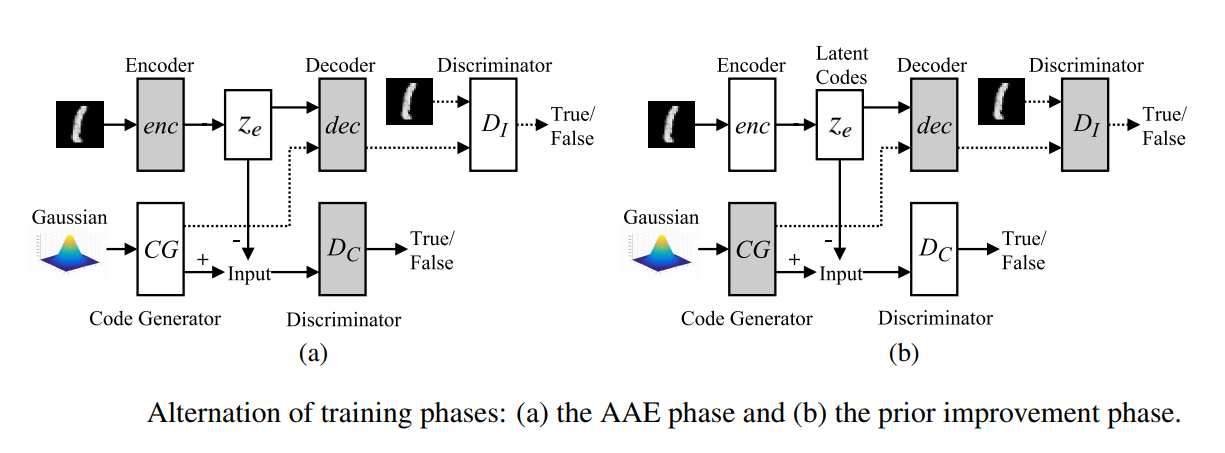
\includegraphics[width=1\textwidth]{figures/original.png}
        \caption{Original paper algorithm scheme}
    \end{figure}

    \subsection{Original paper algorithm pseudo code}
    \begin{figure}[!h]
        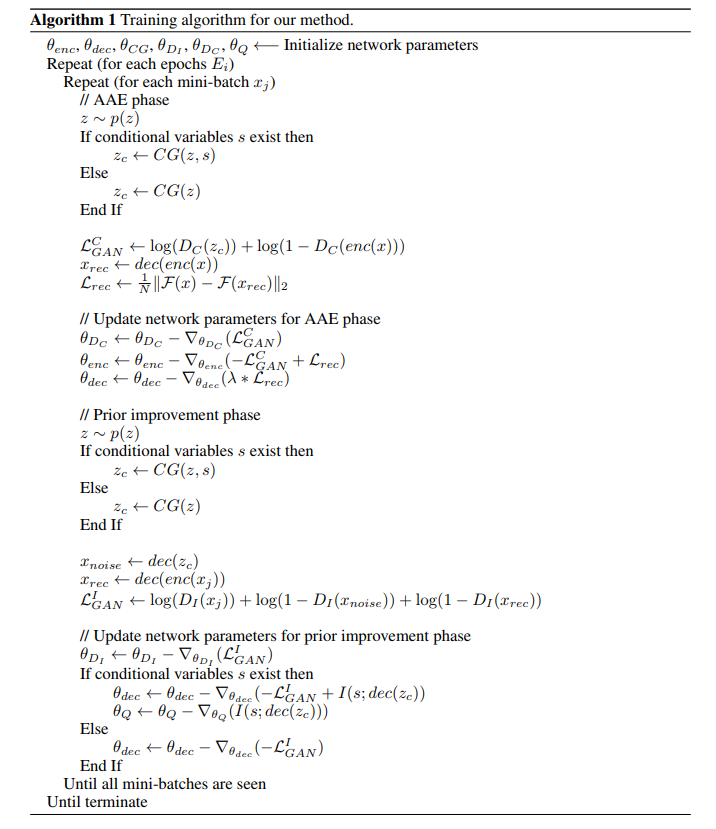
\includegraphics[width=0.6\textwidth]{figures/original-code.png}
        \caption{Original paper algorithm pseudo code}
    \end{figure}


    \subsection{Additional algorithm}
    Is inspired by

    "Autoencoding beyond pixels using a learned similarity metric"\cite{DBLP:journals/corr/LarsenSW15}
    % Commands to include a figure:
    \begin{figure}[!h]
        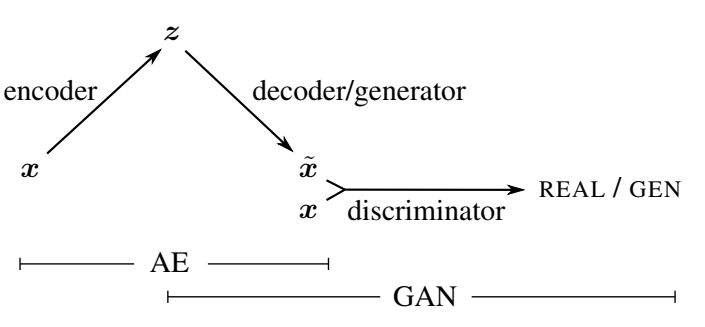
\includegraphics[width=\textwidth]{figures/additional.png}
        \caption{Additional algorithm scheme}
    \end{figure}


    \subsection{Additional algorithm pseudo code}
    \begin{figure}[!h]
        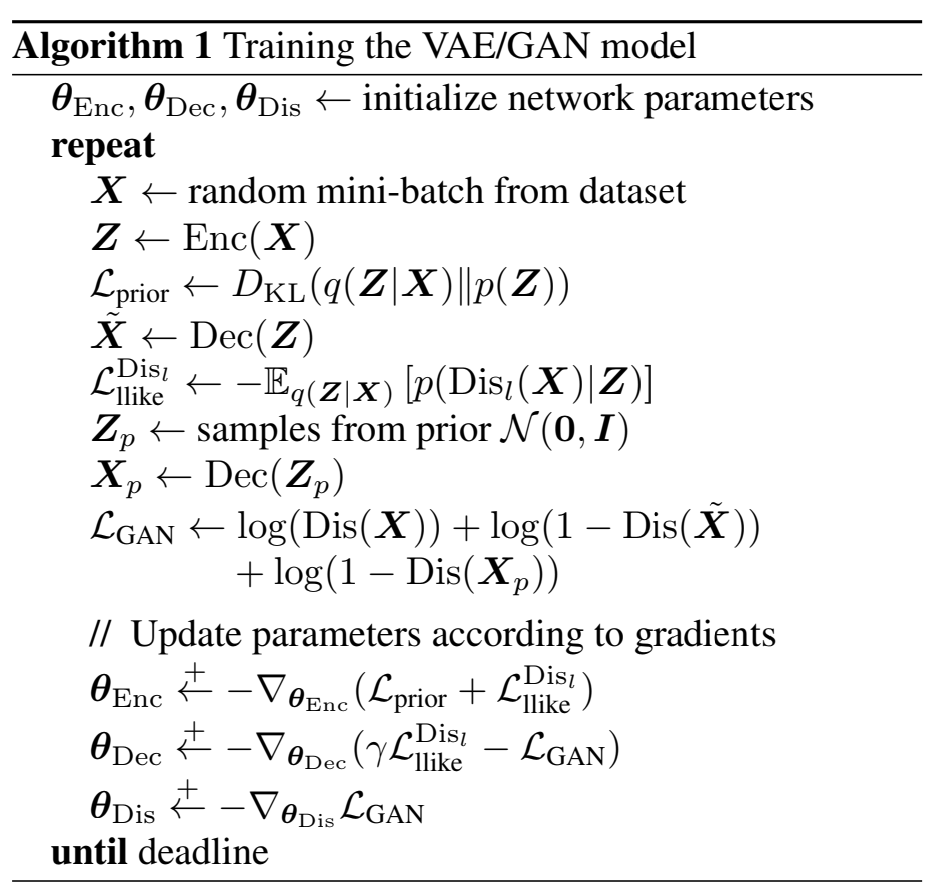
\includegraphics[width=0.7\textwidth]{figures/additional-code.png}
        \caption{Additional algorithm pseudo code}
    \end{figure}


    \section{Data}

    \begin{itemize}
        \item MNIST
        \item CIFAR-10
    \end{itemize}


    \section{Problems and solutions}

    Problems
    \begin{itemize}
        \item Different formulae in the text and the pseudo code in the original paper
        \item 1 epoch even for MNIST takes about 17 minutes
        \item We had no time to try supervised setting
    \end{itemize}
    Solutions
    \begin{itemize}
        \item Using other papers and do updates according to the our own understanding
        \item Several updates of encoder-decoder
        \item Adjusting learning rates
    \end{itemize}


    \section{Results}

    \subsection{Results for AAE}
    Sasha put here your pictures

    \subsection{Results evolution for original paper. MNIST.}
    The most enchanting thing here is evolution with epochs
    \begin{figure}[!h]
        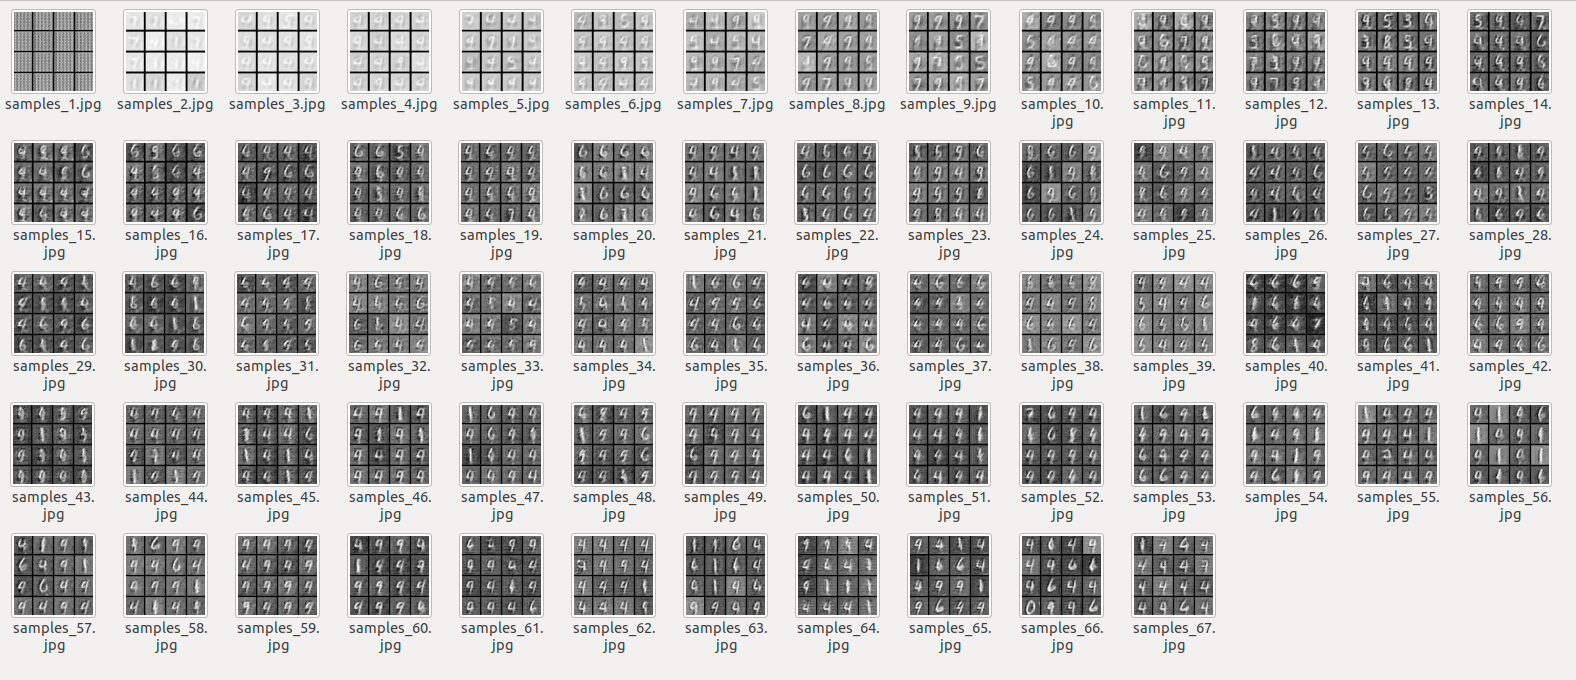
\includegraphics[width=\textwidth]{figures/MNIST-original-evolution.png}
        \caption{Results evolution for original paper. MNIST}
    \end{figure}

    \subsection{Results for original paper. MNIST, 67 epoch.}
    \begin{figure}[!h]
        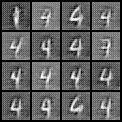
\includegraphics[width=0.7\textwidth]{figures/samples_67.jpg}
        \caption{Results for original paper. MNIST, 67 epoch}
    \end{figure}

    \subsection{Results evolution for original paper. CIFAR.}
    The results are not good at all. Here the latent dimension is 8 the same as for MNIST.
    \begin{figure}[!h]
        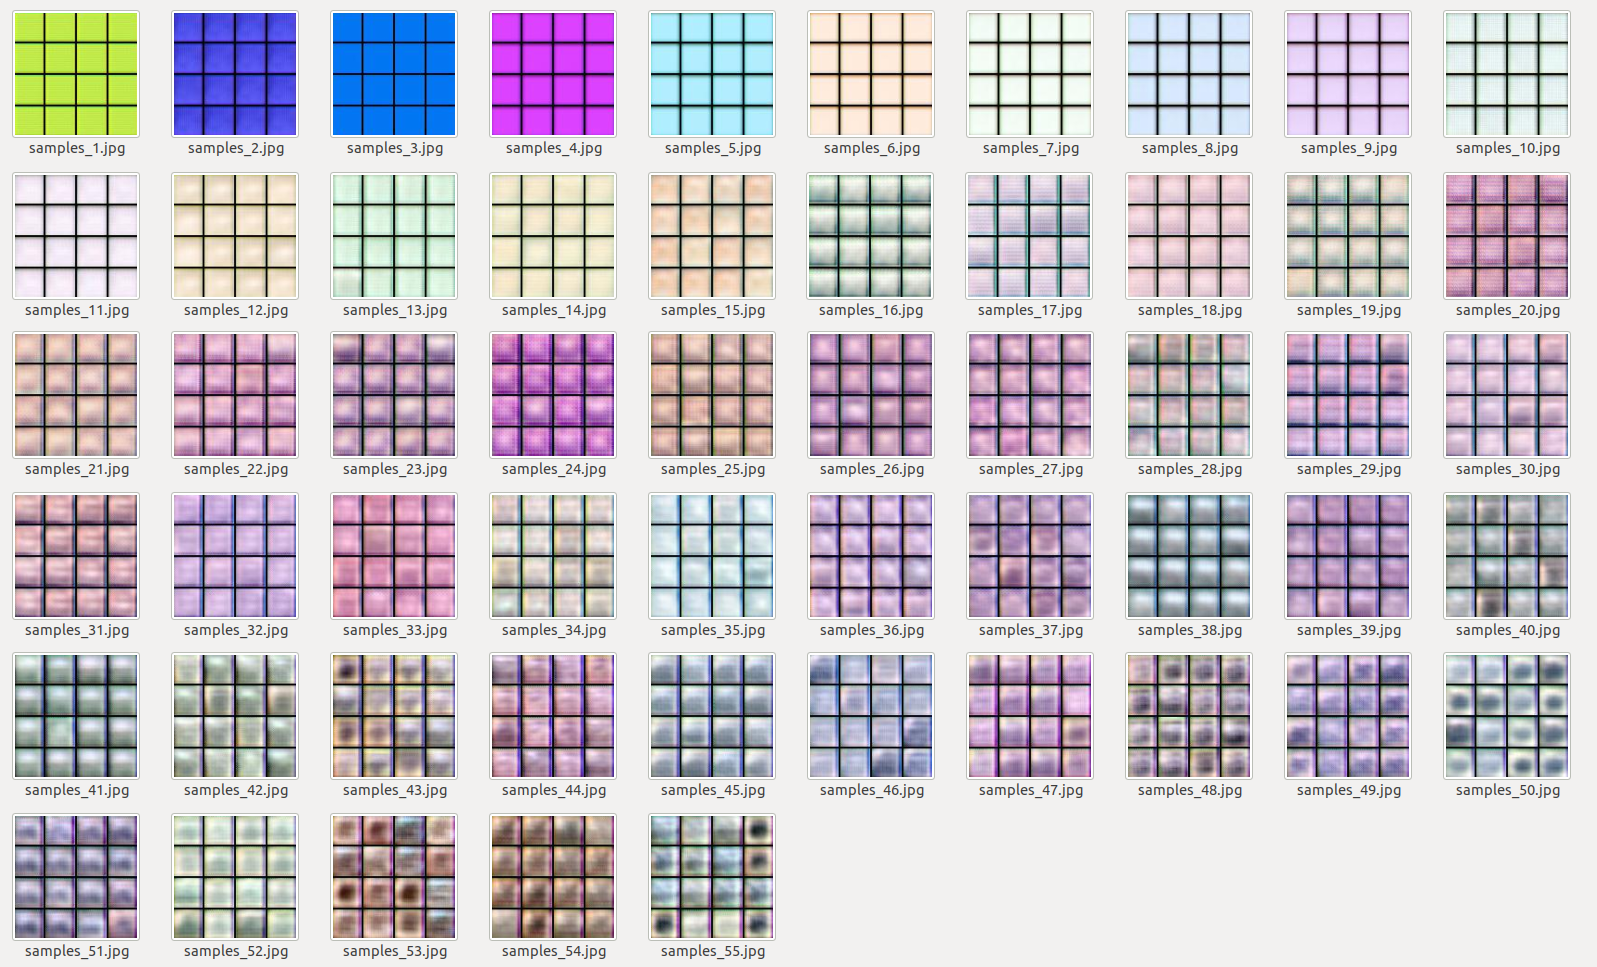
\includegraphics[width=\textwidth]{figures/CIFAR-original-evolution.png}
        \caption{Results evolution for original paper. CIFAR}
    \end{figure}

    \subsection{Results for original paper. CIFAR, 55 epoch.}
    \begin{figure}[!h]
        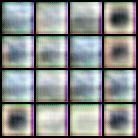
\includegraphics[width=0.7\textwidth]{figures/samples_55.jpg}
        \caption{Results for original paper. CIFAR, 55 epoch}
    \end{figure}

    \subsection{Results for additional algorithm}
    \begin{figure}[!h]
        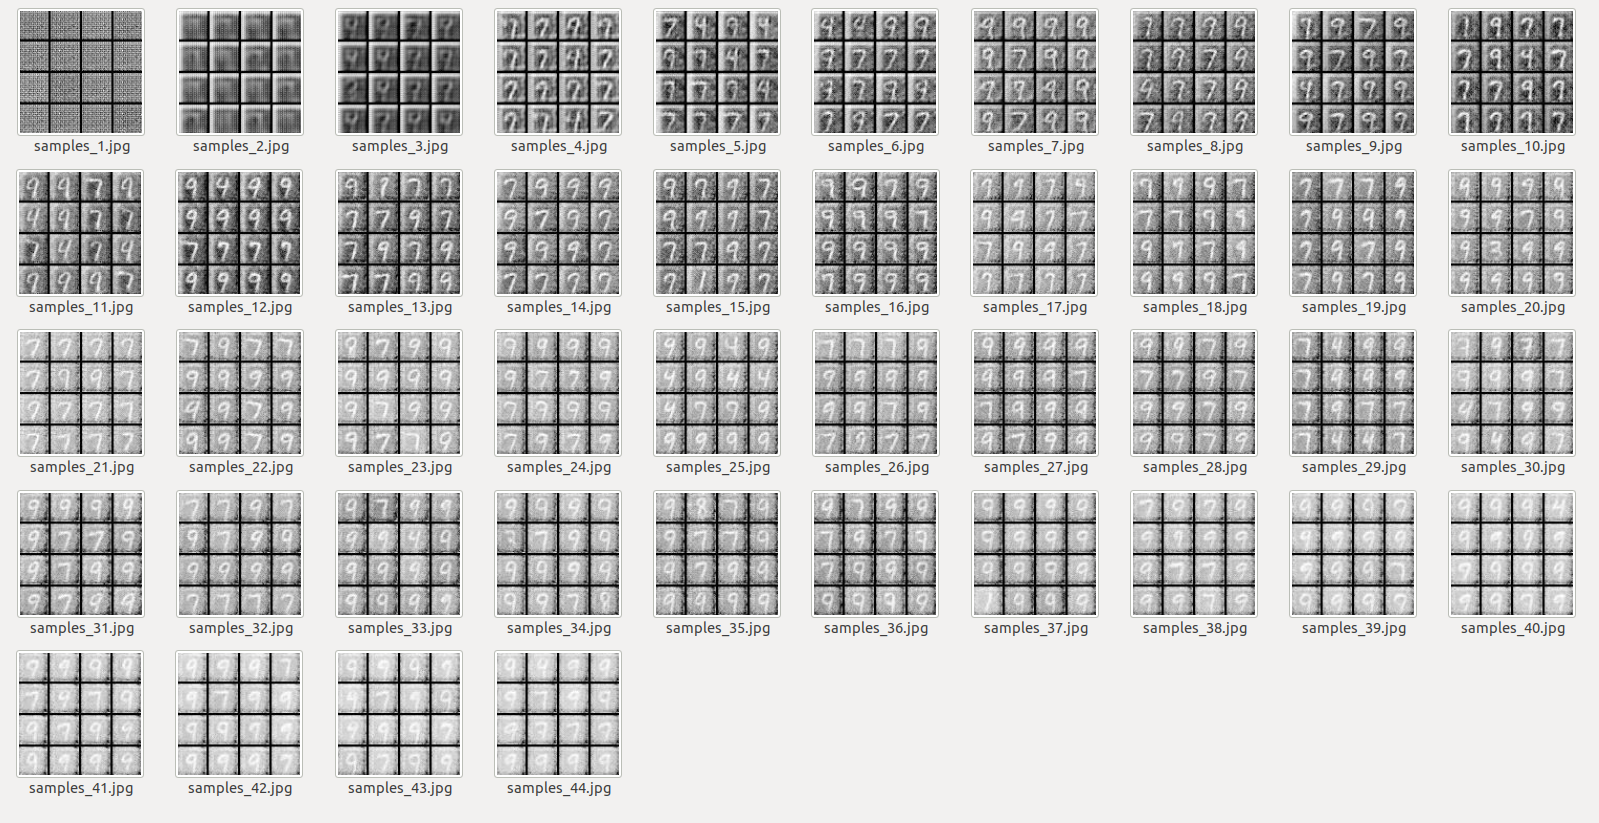
\includegraphics[width=\textwidth]{figures/MNIST-additional-evolution.png}
        \caption{Results evolution for additional algorithm. MNIST}
    \end{figure}

    \subsection{Conclusions}
    \begin{itemize}
        \item The adversarial training is difficult
        \item There are a lot of different schemes of generative models combining GAN and VAE
    \end{itemize}

    \subsection{Contributions}
    \begin{itemize}
        \item Belozerova Polina: reading papers
        \item Safin Alexander: reading papers, implement the classical AAE,
        experiments for MNIST, corresponding parts inthe presentation and report
        \item Pavlovskaia Natalia: reading papers, implement the original paper, implement the additional algorithm,
        experiments for MNIST and CIFAR-10, corresponding parts inthe presentation and report
    \end{itemize}

    \bibliographystyle{unsrt}
    \bibliography{references}

\end{document}
